\documentclass[12pt, a4paper]{article}

\usepackage[top=1in, bottom=1in, left=1.25in, right=1in]{geometry}
\usepackage{mathptmx} % Times New Roman
\usepackage{setspace}
\usepackage{titlesec}
\usepackage{graphicx}
\usepackage{caption}
\usepackage{float}
\usepackage{hyperref}
\usepackage{xurl}
\usepackage{pgfgantt}
\usepackage{tocloft}
\usepackage{parskip}
\usepackage{booktabs}
\usepackage{amsmath}
\usepackage{amssymb}

% TOC dots for all levels
\renewcommand{\cftsecleader}{\cftdotfill{\cftdotsep}}

% Page number bottom centered
\usepackage{fancyhdr}
\fancypagestyle{plain}{
  \fancyhf{}
  \renewcommand{\headrulewidth}{0pt}
  \fancyfoot[C]{\thepage}
}
\pagestyle{plain}

% Line spacing globally
\onehalfspacing

% Headings Configuration
\titleformat{\section}{\normalfont\fontsize{16}{19.2}\bfseries\selectfont}{\thesection.}{1em}{}
\titleformat{\subsection}{\normalfont\fontsize{14}{16.8}\bfseries\selectfont}{\thesubsection}{1em}{}
\titleformat{\subsubsection}{\normalfont\fontsize{12}{14.4}\bfseries\selectfont}{\thesubsubsection}{1em}{}

% Captions Configuration
\DeclareCaptionFont{twelvept}{\fontsize{12}{14.4}\selectfont}
\captionsetup[figure]{font={bf,twelvept}, labelsep=colon, justification=centering, position=bottom}

\begin{document}
\pagenumbering{roman}

% Cover Page
\begin{titlepage}
\begin{singlespace}
\begin{center}
\vspace*{0.1cm}
{\fontsize{16}{19.2}\bfseries Kathford International College of Engineering and Management\\}
\vspace{0.2cm}
{\fontsize{14}{16.8}\bfseries Balkumari, Lalitpur, Nepal\\}

\vspace{0.5cm}

\includegraphics[width=4cm]{kathford_logo.jpg}\\

\vspace{0.6cm}
{\fontsize{14}{16.8}\bfseries A\\}
\vspace{0.3cm}
{\fontsize{16}{19.2}\bfseries Project Proposal\\}
\vspace{0.3cm}
{\fontsize{14}{16.8}\bfseries on\\}
\vspace{0.5cm}
{\fontsize{16}{19.2}\bfseries PERSONAL FINANCE MANAGER (PFM)\\}

\vspace{0.8cm}
{\fontsize{14}{16.8}\bfseries Submitted To\\}
\vspace{0.4cm}
{\fontsize{12}{14.4} Department of Information Technology\\}
\vspace{0.2cm}
{\fontsize{12}{14.4} Kathford International College of Engineering and Management\\}

\vspace{1.2cm}
{\fontsize{12}{14.4}\bfseries In partial fulfillment of the requirement for the Bachelor Degree in Computer Application\\}

\vspace{1.2cm}
{\fontsize{14}{16.8}\bfseries Submitted By\\}
\vspace{0.4cm}
{\fontsize{12}{14.4} Gaurav Kr Sah (6-2-456-112-2021)\\}
\vspace{0.2cm}
{\fontsize{12}{14.4} Nirmal Sapkota (6-2-456-123-2021)\\}

\end{center}
\end{singlespace}
\end{titlepage}

\newpage
\renewcommand{\contentsname}{\centerline{\fontsize{16}{19.2}\normalfont\bfseries TABLE OF CONTENTS}}
\tableofcontents
\newpage

\pagenumbering{arabic}
\setcounter{page}{1}

% ─────────────────────────────────────────────────────────────────────────────
\section{Introduction}

Most students know the frustration of checking their bank balance and wondering where the money went. During our fourth semester, we tracked daily expenses in a shared Google spreadsheet. We quit after six days. The problem was not the spreadsheet; it was stopping mid-day to open a laptop, find the file, and type a new row for every small purchase. That kind of habit is genuinely hard to build.

Existing finance apps do not solve this well. Splitwise, Wallet, and similar tools all share the same friction: they are form-driven. To record a transaction you tap through menus, pick a category from a list, and enter numbers manually. The interface is cleaner than a spreadsheet, but the effort is the same. People download these apps with good intentions and stop using them within a few weeks.

The Personal Finance Manager (PFM) will take a different approach. Instead of presenting forms, the system accepts plain text. A user can type something like ``paid 500 for lunch'' and the application handles the rest: find the amount, figure out the date, assign a category, and store the record. No menus. No mandatory fields.

This is our final year project for the Bachelor of Computer Applications degree at Tribhuvan University. The T.U. guidelines require a system that goes beyond basic database operations and demonstrates working algorithms written by the students themselves \cite{tuguide}. The core of PFM will be a custom NLP text parsing pipeline, a greedy algorithm for budget optimization, and a RAG-based financial query module, all running on our own server.

\newpage
% ─────────────────────────────────────────────────────────────────────────────
\section{Problem Statement}

The core problem is not a shortage of finance apps. There are plenty. The problem is that none of them stay part of a person's daily routine. Three specific issues drive this:

\begin{itemize}
    \item Manual data entry is where most people give up. Every existing tracker expects the user to pick a category, fill in an amount, and add a date for every single purchase. That is enough friction that most users stop logging after a few days. The tool that is supposed to help becomes another chore.

    \item Category assignment is too rigid. Apps that auto-classify transactions use keyword lists or fixed rules. A transaction labeled ``team lunch'' ends up filed as Food when it probably belongs under Business. Keyword logic cannot resolve context. A better approach is a trained probabilistic parser that understands input more flexibly.

    \item There is no useful budget guidance. Most apps let you set a spending limit manually but do not tell you how to distribute money across categories given your actual history. Users are left guessing. An optimization algorithm can do this work automatically.

    \item Student projects limited to create-read-update-delete operations miss the analytical dimension that the T.U. guidelines specifically ask for \cite{tuguide}. PFM addresses this by building a genuine NLP parsing engine, a greedy budget optimizer, and a RAG-based query system that form the analytical backbone of the application.
\end{itemize}

\newpage
% ─────────────────────────────────────────────────────────────────────────────
\section{Objectives}

The outcomes we are working toward:

\begin{itemize}
    \item To design and implement a custom NLP parsing pipeline in Python that accepts free-form expense text, extracts the amount and description, detects context like loan repayments or income, and assigns a category using a large keyword-based classifier we build ourselves.
    \item To build a greedy budget optimizer in JavaScript that reads a user's spending history by category and suggests how to trim the budget, cutting non-essential categories first and essential ones only as a last resort.
    \item To implement a RAG (Retrieval-Augmented Generation) service that groups historical transactions by month and year and passes them as context to the Gemini API, enabling natural language queries like ``how much did I spend on food in March?''
    \item To build a FastAPI \cite{fastapi} backend that exposes all modules as REST endpoints with JWT-based authentication and row-level data isolation via Supabase \cite{supabase}.
    \item To build a React \cite{react} dashboard showing spending summaries, category breakdowns, the budget optimizer, and a transaction table with filtering.
\end{itemize}

The core commitment is that the NLP parser and budget optimizer will be written by us, not assembled from third-party classification APIs or optimization libraries. The Gemini API \cite{gemini} handles two narrow roles: answering natural language financial queries over the user's own data, and categorizing expense descriptions that do not match any keyword in our parser. Both are controlled API calls, not open-ended generation.

\newpage
% ─────────────────────────────────────────────────────────────────────────────
\section{Methodology}

\subsection{Requirement identification}

\subsubsection{Study of existing systems}

We reviewed two widely used personal finance applications to understand what gaps PFM will fill.

Splitwise is built for group expense splitting, not personal budgeting. It has no monthly trend tracking, no category breakdown for individual users, and no way to forecast from past records. Every transaction assumes multiple people, which is not useful for a student managing their own finances.

Wallet by Budget Bakers offers analytical charts and budget planning. The data entry process is identical to most competitors: open a form, fill in an amount, select a category from a dropdown, add a note, and save. The interface is polished, but the workflow demands the same manual effort that drives high abandonment. Bank sync features are behind a paywall and are not available for most Nepali banks.

Neither application processes natural language input. Neither suggests budget allocations based on history.

\subsubsection{Literature review}

Text classification using statistical models is a well-studied area. Sebastiani (2002) \cite{sebastiani} established the foundation for using probabilistic models to assign documents to predefined categories, a technique applicable to classifying expense descriptions. Naive Bayes classifiers are effective for short text because they handle sparse feature vectors well.

TF-IDF (Term Frequency-Inverse Document Frequency) converts raw text into numerical vectors that capture how strongly a term indicates a specific category \cite{manning}. Words like ``petrol'' are rare enough across the corpus to carry strong signal for the Transport category; words like ``paid'' appear everywhere and contribute little.

For budget allocation with a fixed total and multiple categories, a greedy approach based on historical spending ratios is both simple to implement and easy for users to understand.

RAG (Retrieval-Augmented Generation) combines a retrieval step with a language model. Instead of asking a language model to answer from memory, RAG provides it with specific context documents, in our case, the user's actual transaction history grouped by time period \cite{gemini}. This keeps responses grounded in real data.

\subsubsection{Requirement analysis}

Functional requirements:
\begin{itemize}
    \item Accept raw text input and extract the transaction amount, category, and description through a custom NLP pipeline.
    \item Detect and handle diverse input patterns including loan transactions, income entries, ambiguous transfers between people, and multi-item entries separated by commas.
    \item Authenticate users and isolate their data at the database row level.
    \item Store parsed transactions in a PostgreSQL table linked to the authenticated user.
    \item Run a greedy algorithm to suggest spending cuts when the user sets a savings target.
    \item Accept natural language queries about past spending and return accurate answers using the RAG module.
    \item Fall back to Gemini for category prediction only when the local keyword parser returns no match.
\end{itemize}

Non-functional requirements:
\begin{itemize}
    \item End-to-end processing from text submission to dashboard refresh should complete within three seconds under normal network conditions.
    \item The parser should correctly classify at least 80 percent of typical expense inputs without any Gemini fallback.
    \item The interface must be responsive and usable on mobile browsers without a dedicated native app.
    \item All user data must be row-level isolated. No user can access another user's records.
\end{itemize}

\subsection{Feasibility study}

\subsubsection{Technical feasibility}

Both team members have completed coursework in Python, web development, and database management through the seventh semester. The NLP pipeline will use Python's regular expression engine and a custom keyword dictionary we build ourselves. FastAPI \cite{fastapi} will provide the async API server. The frontend will be built with React 18 and Vite, both of which we have used in previous work.

The technology stack:
\begin{itemize}
    \item Python 3.11 for the backend language, NLP parsing scripts, and algorithm implementations.
    \item FastAPI \cite{fastapi} for the REST API framework, chosen for its native async support and auto-generated documentation.
    \item React 18 with Vite for the frontend single-page application.
    \item Recharts for rendering spending charts.
    \item Supabase \cite{supabase} for the PostgreSQL database, authentication, and row-level security.
    \item Google Gemini API \cite{gemini} for the RAG query module and category fallback.
\end{itemize}

\subsubsection{Operational feasibility}

The primary user interface is a single text input. Typing a short sentence about a purchase requires no tutorial and no knowledge of accounting. If a user can send a text message, they can use PFM. The budget optimizer requires entering one number (a total monthly target), and the algorithm handles the allocation. This makes the system genuinely usable for students who have little patience for complex financial software.

\subsubsection{Economic feasibility}

The full system runs at zero cost during development and initial deployment.

Frontend hosting on CPanel: The React application compiles to static files (HTML, CSS, JavaScript) that Apache on our existing shared hosting server can serve without additional cost.

Backend hosting on Render: The FastAPI backend is deployed as a web service on Render's free tier, which provides sufficient uptime for development and demonstration.

Database on Supabase: The free tier includes a PostgreSQL database with 500~MB of storage, built-in authentication, and row-level security. For a personal finance tracker used by a small group during the project period, 500~MB is more than enough.

Gemini API: The free tier provides 1,500 requests per day. Since Gemini is only invoked for RAG queries and uncategorized items, and the local parser handles the vast majority of inputs, actual Gemini usage will stay well within this limit.

Estimated monthly cost during development and testing: NPR 0.

\subsection{Algorithm design plan}

This section describes the three algorithms we will implement ourselves.

\subsubsection{NLP expense parser}

The parser is the core of how PFM understands user input. When a user types something like ``paid 500 for lunch'', the parser does several things in sequence.

First, it normalizes the input: comma-separated numbers like 1,00,000 are cleaned up, and the text is split on commas or the word ``and'' to allow multi-item entries in a single message.

For each segment, the parser then tries to match it against a prioritized list of regular expression patterns. It checks for loan patterns first (things like ``hari lent me 400'', ``repaid sonu 200 from bank''), then income patterns (``got salary 50000''), and finally falls through to a general ``amount item'' pattern that handles the common case.

Category assignment happens through a large keyword dictionary we maintain. Each category (Food, Transport, Groceries, Shopping, Utilities, etc.) has a curated list of keywords including Nepali terms and common abbreviations. The parser checks the decoded item text against these lists and picks the first match. If no keyword matches, the system calls the Gemini fallback to infer a category from context, returning only a category label.

The parser also handles ambiguous person-based transactions, where the intent (loan versus gift versus payment) is unclear, by flagging them for user confirmation in the UI.

\subsubsection{Greedy budget optimizer}

The budget optimizer is a frontend module. When a user enters a target monthly savings amount, the algorithm calculates how much needs to be cut from their current spending and then works through spending categories from highest to lowest.

Non-essential categories (entertainment, shopping, etc.) are cut first, up to 50 percent of their current amount per category. If that is still not enough, essential categories (rent, food, medical) are trimmed by a smaller margin of 10 percent.

The result is a list of specific suggested cuts per category, totaling as close to the savings target as possible. The algorithm terminates when either the target is met or all categories have been reduced to their floors.

This is written as a pure JavaScript function in the frontend utility layer, with no external optimization library.

\subsubsection{RAG financial query module}

The RAG module answers natural language questions about the user's spending history. When a user asks something like ``how much did I spend on transport last month?'', the backend retrieves the user's transactions from Supabase, groups them by year and month, and builds a structured context document that includes all-time totals, yearly breakdowns, monthly breakdowns, category distributions, and loan summaries by person.

This context is passed to the Gemini API along with the user's question and a prompt that instructs Gemini to answer only from the provided data, use exact figures, and format currency as Rs.X. Gemini returns a plain text answer that the chat interface displays directly.

If Gemini is unavailable or the API key is missing, the system falls back to a local pattern-matching query engine in the backend that handles common question types without calling any external service.

\subsection{High level design of system}

PFM is built as a three-tier system: a mobile-responsive React frontend, a FastAPI logic layer, and a Supabase database.

When a user submits an expense in plain text, the React frontend sends it to the FastAPI parser endpoint. The parser applies pattern matching and keyword classification, returns structured transaction objects, and the frontend writes them to the Supabase \texttt{expenses} table. The chat interface also handles conversational queries, routing them to the RAG module which fetches user data from Supabase, builds context, and queries Gemini for a grounded answer.

Analytical features including the budget optimizer and the moving average trend chart run in the frontend on data already loaded from Supabase, keeping those interactions fast without additional API requests.

\begin{figure}[H]
    \centering
    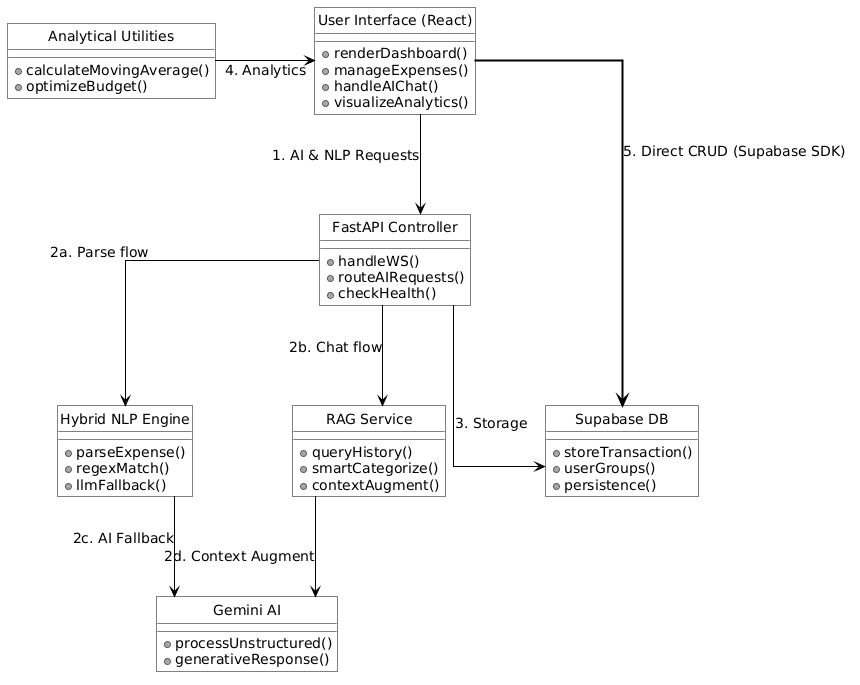
\includegraphics[width=1.0\textwidth]{hld.png}
    \caption{High-level system architecture (tiered design)}
\end{figure}

\begin{figure}[H]
    \centering
    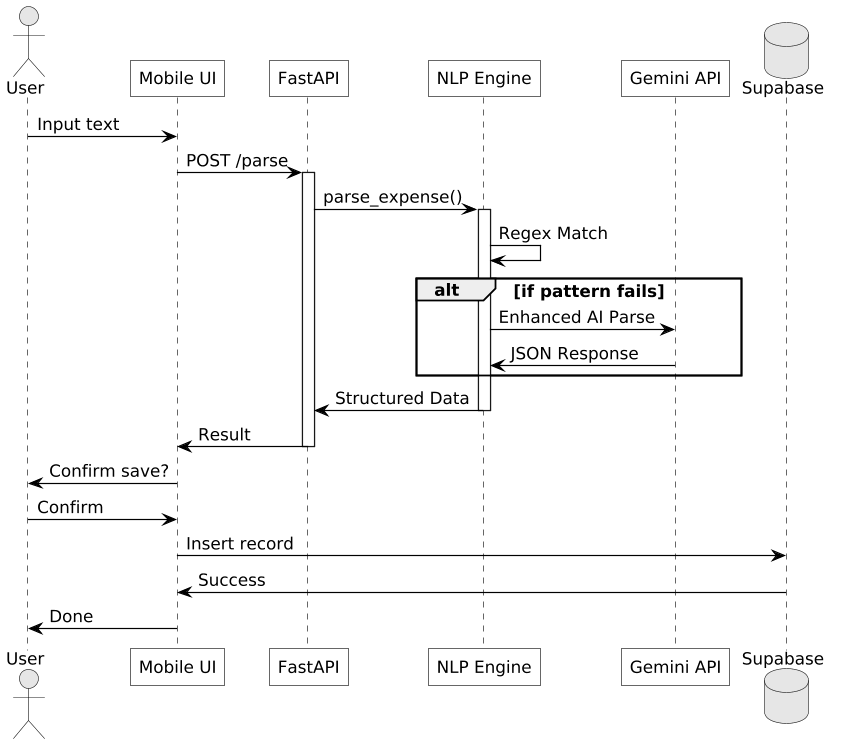
\includegraphics[width=0.85\textwidth]{sequence.png}
    \caption{Sequence diagram: hybrid expense classification process}
\end{figure}

\newpage
% ─────────────────────────────────────────────────────────────────────────────
\section{Gantt Chart}

The planned timeline runs eighteen weeks from mid-March to late July 2026. Algorithm implementation (the NLP parser and the greedy optimizer) is allocated the longest window because it is the part most likely to require iteration.

\begin{figure}[H]
    \centering
    \begin{ganttchart}[
        x unit=0.55cm,
        y unit title=0.6cm,
        y unit chart=0.6cm,
        vgrid,
        hgrid,
        title label anchor/.style={below=-1.5ex},
        title height=1,
        bar/.style={fill=black!60},
        bar label font=\footnotesize,
        title label font=\footnotesize,
        progress label text={},
        bar height=0.6
      ]{1}{18}
      \gantttitle{Mar}{2} \gantttitle{Apr}{4} \gantttitle{May}{4} \gantttitle{Jun}{4} \gantttitle{Jul}{4} \\
      \gantttitlelist{3,4, 1,2,3,4, 1,2,3,4, 1,2,3,4, 1,2,3,4}{1} \\
      \ganttbar{System Study \& Lit. Review}{1}{3} \\
      \ganttbar{Requirement Gathering}{2}{4} \\
      \ganttbar{Architecture \& DB Design}{4}{6} \\
      \ganttbar{Backend Core Dev (FastAPI)}{6}{10} \\
      \ganttbar{NLP Parser \& Greedy Optimizer}{8}{13} \\
      \ganttbar{Frontend Interface (React)}{10}{14} \\
      \ganttbar{System Integration \& Testing}{13}{16} \\
      \ganttbar{Report Writing \& Defense}{16}{18}
    \end{ganttchart}
    \caption{Project timeline: March to July 2026}
\end{figure}

\newpage
% ─────────────────────────────────────────────────────────────────────────────
\section{Expected Outcome}

At the end of the project, we expect to deliver a working web application where:

\begin{itemize}
    \item A user can type any expense in plain English or common Nepali terms and have it categorized and stored without filling any form.
    \item The local NLP parser handles at least 80 percent of inputs correctly on its own. The Gemini fallback covers the rest, keeping overall accuracy above 90 percent.
    \item The budget optimizer returns specific suggested cuts per category derived from the user's own spending history.
    \item The RAG chat interface correctly answers natural language queries about past spending, including time-filtered questions like ``what did I spend in February?''
    \item The full flow from text input to dashboard update completes within three seconds under normal network conditions.
\end{itemize}

As a final year project under the T.U. BCA 8th semester guidelines \cite{tuguide}, PFM demonstrates the implementation of custom logic modules rather than reliance on black-box plugins. The NLP parser, the greedy budget optimizer, and the RAG query module are the core evidence of this. Gemini handles two specific, bounded tasks: answering contextual financial queries and providing category labels for inputs the local parser cannot classify.

\newpage
% ─────────────────────────────────────────────────────────────────────────────
\section{References}

\begin{thebibliography}{99}

\bibitem{fastapi}
Ramirez, S. (n.d.). \textit{FastAPI Documentation.} Retrieved from \url{https://fastapi.tiangolo.com/}

\bibitem{react}
Facebook Inc. (n.d.). \textit{React: A JavaScript library for building user interfaces.} Retrieved from \url{https://react.dev/}

\bibitem{gemini}
Google LLC. (2024). \textit{Gemini API Documentation.} Retrieved from \url{https://ai.google.dev/}

\bibitem{supabase}
Supabase Inc. (n.d.). \textit{Supabase: Open source Firebase alternative with PostgreSQL.} Retrieved from \url{https://supabase.com/docs}

\bibitem{sebastiani}
Sebastiani, F. (2002). Machine learning in automated text categorization. \textit{ACM Computing Surveys}, 34(1), 1--47. \url{https://doi.org/10.1145/505282.505283}

\bibitem{manning}
Manning, C. D., Raghavan, P., \& Schuetze, H. (2008). \textit{Introduction to Information Retrieval.} Cambridge University Press. Retrieved from \url{https://nlp.stanford.edu/IR-book/}

\bibitem{tuguide}
Tribhuvan University, Faculty of Humanities and Social Sciences. (2023). \textit{BCA 8th Semester Project Guidelines.} Kathmandu: T.U. Publications.

\end{thebibliography}

\end{document}
